\section{Design Space for the Orchestration Function} % and orchestration function

\mnote{Undefined when application function is expected to return consistent models}
To recapitulate, the definition of an application function for transformation networks, given in \autoref{def:applicationfunction}, requires an application function $\appfunction{\orcfunction{\transformationset{T}}}$ to accept models and changes to them and yields either a set of models or $\bot$.
Whenever it returns a set of models, they must be achieved by applying the transformations in $\transformationset{T}$ of the network in an order determined by the orchestration function $\orcfunction{\transformationset{T}}$.
We then say that this execution order is an \emph{orchestration} of the transformations and that the execution of transformations in that order \emph{yields} those models.
The notion of correctness for the application function given in \autoref{def:applicationfunctioncorrectness} additionally requires the returned models to be consistent.
We did, however, not yet define when we expect the function to return consistent models and when we allow it to return $\bot$, as this requires further discussion of the alternatives, which we make in the following.

\mnote{Application function highly depends on orchestration function}
In fact, the application function highly depends on the results of the orchestration function.
If that function does not deliver an orchestration that yields consistent models, a correct application function may only return $\bot$.
Thus, we are specifically concerned with ensuring that the orchestration function finds an orchestration that yields consistent models as often as possible.
We call an orchestration that yields consistent models a \emph{consistent orchestration}.
Precisely, we define an orchestration and a consistent orchestration as follows.

\begin{definition}[Orchestration]
    Let $\transformationset{T}$ be a set of transformation.
    We call any sequence of those transformations $\tupled{\transformation{t}_{1}, \transformation{t}_{2}, \dots} \in \transformationset{T}^{< \mathbb{N}} \equalsperdefinition \emptyset \cup \transformationset{T}^1 \cup \transformationset{T}^2 \cup \dots$ an \emph{orchestration} of them.

    For models $\modeltuple{m} \in \metamodeltuple{M}$ and changes $\changetuple{\metamodeltuple{M}} \in \changeuniverse{\metamodeltuple{M}}$, we say that an orchestration $\tupled{\transformation{t}_{1}, \dots, \transformation{t}_{n}}$ is \emph{consistent} if, and only if, the subsequent application of the transformations to $\modeltuple{m}$ and $\changetuple{\metamodeltuple{M}}$  is consistent, i.e., $\generalizationfunction{\metamodeltuple{M},\transformation{t}_{n}} \concatfunction \dots \concatfunction \generalizationfunction{\metamodeltuple{M},\transformation{t}_{1}}(\modeltuple{m}, \changetuple{\metamodeltuple{M}}) \consistenttomath \transformationset{T}$.
\end{definition}

\mnote{Orchestration function is allowed to return arbitrary long sequences of transformations}
The definition of an orchestration function allows it to determine an arbitrary long sequence of transformations, also including each transformation multiple times.
While we introduced this general notion to avoid unnecessary restrictions, in the following we show the necessity of having this general notion, rather than allowing each transformation to be executed only once, as proposed by existing work, such as \cite{stevens2020BidirectionalTransformationLarge-SoSym}.
From the insight that we need to allow transformations to be executed multiple times, we derive and discuss when we expect the application function to return consistent models, to finally come up with a notion of \emph{optimality} for the orchestration function determining the execution order.

% Discuss options for realizing the functions:
% Orchestration returns only sequence with each transformation executed once vs. arbitrary number of executions

% \begin{itemize}
%     \item We introduced a transformation network as a set of transformations, and an application function that uses an orchestration function to determine the execution order of the transformations for a given input
%     \item An application function may return $\bot$ or consistent models to be correct.
%     \item It may always return $\bot$ to be correct, this is however not what we want.
%     \item It would be intuitive to expect an application function to always return consistent models when there is an execution order of the transformations (i.e. an orchestration) that delivers consistent models.
%     \item So, we first investigate whether we can define a bound for the number of necessary transformation executions.
%     \item We there conclude, that we cannot restrict the number of necessary transformation execution
% \end{itemize}


\subsection{Single Transformation Execution}

\mnote{Ranges for possible numbers of transformation executions}
The possible number of executions for transformations of network range from a selected execution, e.g., in terms of spanning tree, over the execution of each transformation for one or a fixed number of times, to an arbitrary number of executions per transformations.
In the following, we will motivate why the single execution of each transformation is not sufficient in practice and prove that there can be cases in which it is not sufficient.

\mnote{Spanning trees are not sufficient}
The even stronger restriction to spanning trees is obviously not sufficient.
Consider the following consistency relations. For reasons of simplicity, we use \modellevelconsistencyrelations instead of fine-grained relations:
\begin{align*}
    & 
    \consistencyrelation{CR}{12} = \setted{\tupled{\model{m}{1}, \model{m}{2}}, \tupled{\model{m}{1}, \model{m}{2}'}, \tupled{\model{m}{1}', \model{m}{2}'}, \tupled{\model{m}{1}', \model{m}{2}''}} \\
    & 
    \consistencyrelation{CR}{13} = \setted{\tupled{\model{m}{1}, \model{m}{3}}, \tupled{\model{m}{1}, \model{m}{3}''}, \tupled{\model{m}{1}', \model{m}{3}}, \tupled{\model{m}{1}', \model{m}{3}'}} \\
    & 
    \consistencyrelation{CR}{23} = \setted{\tupled{\model{m}{2}, \model{m}{3}}, \tupled{\model{m}{2}', \model{m}{3}'}, \tupled{\model{m}{2}', \model{m}{3}''}, \tupled{\model{m}{2}'', \model{m}{3}}} 
\end{align*}
%We consider the set of these relations with their transposed ones: $\consistencyrelationset{CR} = \setted{\consistencyrelation{CR}{12}, \consistencyrelation{CR}{12}^T, \consistencyrelation{CR}{13}, \consistencyrelation{CR}{13}^T, \consistencyrelation{CR}{23}, \consistencyrelation{CR}{23}^T}$.
That set of relations is compatible according to \autoref{def:compatibility}, because for model there is a containing set of models that is consistent.
For the initial tuple of models $\tupled{\model{m}{1}, \model{m}{2}, \model{m}{3}}$, we consider a change that changes $\model{m}{1}$ to $\model{m}{1}'$.
Then we can distinguish tree possibly spanning trees of transformations that try to restore consistency, which we denote with $\transformation{T}_{12}, \transformation{T}_{13}, \transformation{T}_{23}$ for the according consistency relations.
Each tree consists of two transformations.
\begin{properdescription}
    \item[$\transformation{T}_{12}$, $\transformation{T}_{13}$:] 
    $\transformation{T}_{12}$ may change $\model{m}{2}$ to $\model{m}{2}'$. $\transformation{T}_{13}$ does nothing, because $\model{m}{1}'$ and $\model{m}{3}$ are already consistent to $\consistencyrelation{CR}{13}$.
    $\model{m}{2}'$ and $\model{m}{3}$ are, however, not consistent to $\consistencyrelation{CR}{23}$.
    \item[$\transformation{T}_{12}$, $\transformation{T}_{23}$:] 
    Like before, $\transformation{T}_{12}$ may change $\model{m}{2}$ to $\model{m}{2}'$. 
    $\transformation{T}_{23}$ may then change $\model{m}{3}$ to $\model{m}{3}''$. 
    $\model{m}{1}'$ and $\model{m}{3}''$ are, however, not consistent to $\consistencyrelation{CR}{13}$.
    \item[$\transformation{T}_{13}$, $\transformation{T}_{23}$:]
    $\transformation{T}_{13}$ may do nothing, because $\model{m}{1}'$ and $\model{m}{3}$ are already consistent to $\consistencyrelation{CR}{13}$.
    $\transformation{T}_{23}$ does also nothing, because $\model{m}{2}$ and $\model{m}{3}$ are still consistent to $\consistencyrelation{CR}{23}$.
    $\model{m}{1}'$ and $\model{m}{2}$ are, however, not consistent to $\consistencyrelation{CR}{12}$.
\end{properdescription}

\mnote{Each transformation needs to be executed at least once}
Thus, we need to execute each transformation at least once, because each transformation is only responsible for restoring its consistency relations and thus we cannot expect the resulting models to be consistent if some transformation were not executed, although the involved models were changed by other transformations.
However, restricting the execution to each transformation once is not appropriate either.
To show that, we consider examples that we derived from those we have already presented in \owncite{gleitze2020orchestration}, which used a different scenario context.

\begin{figure}
    \centering
    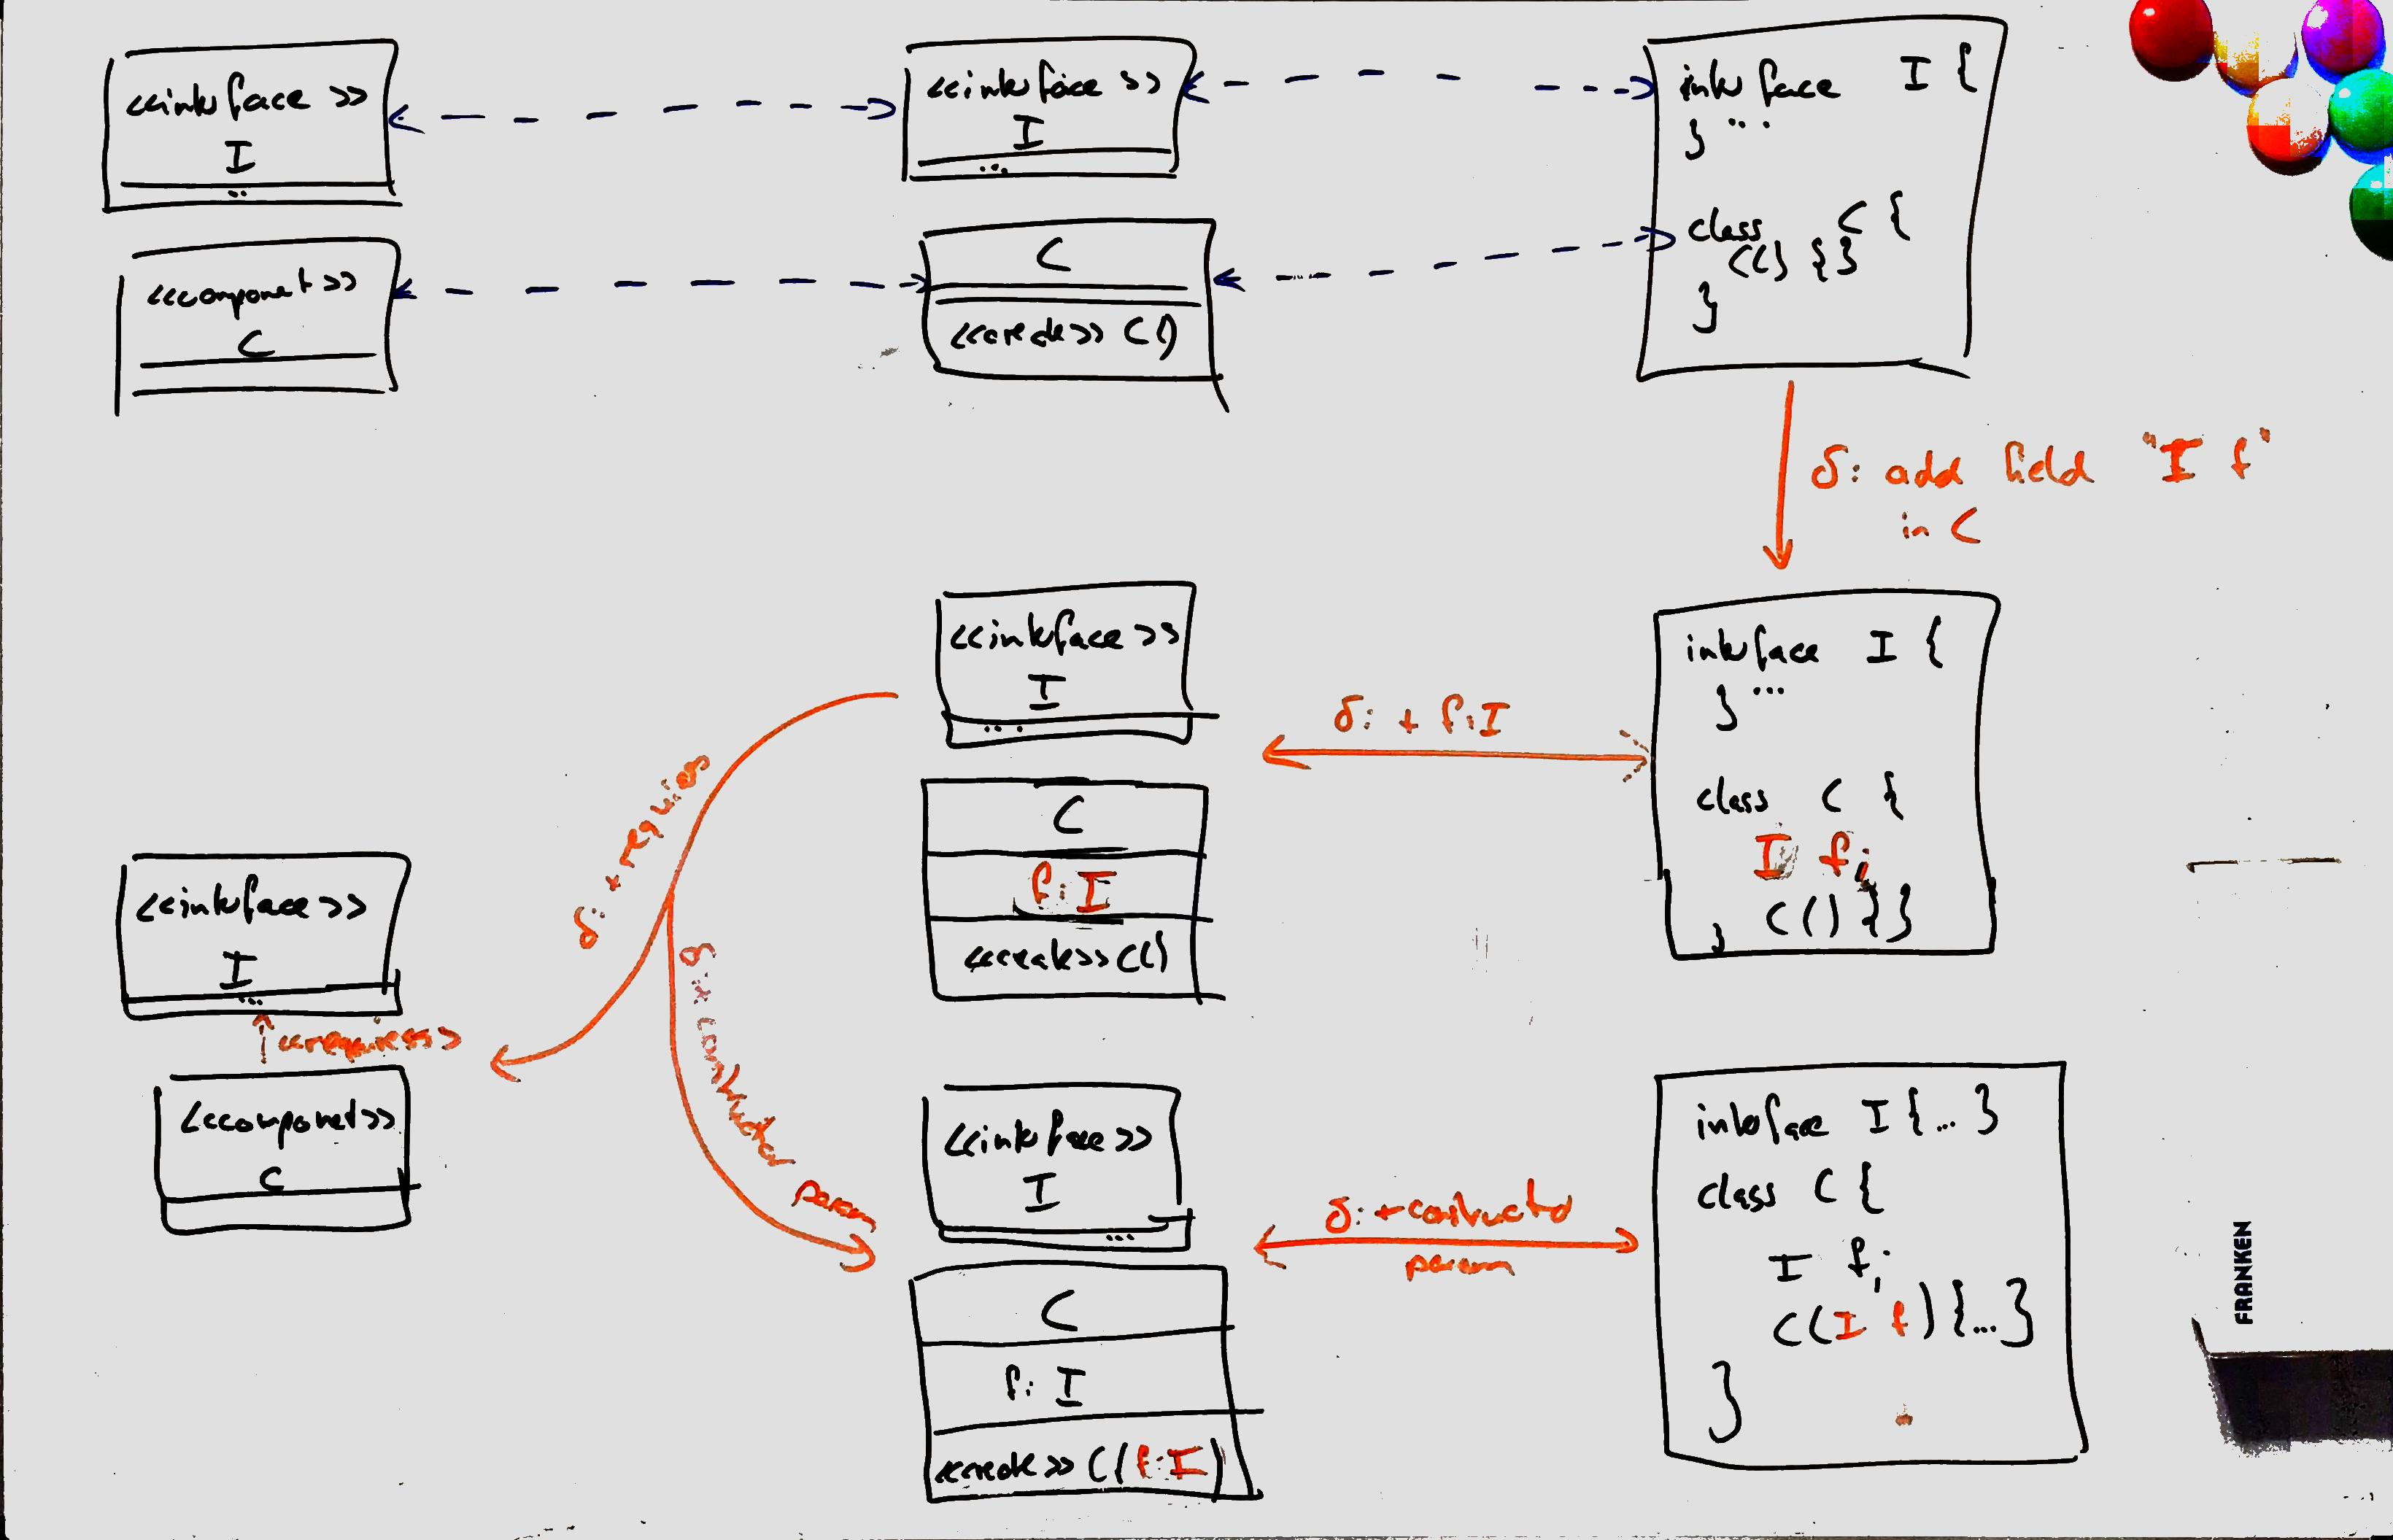
\includegraphics[width=\textwidth]{figures/correctness/orchestration/necessity_multiple_executions.jpg}
    \caption[Necessity of executing a transformation multiple times]{Necessity of executing a transformation multiple times.}
    \label{fig:orchestration:necessity_multiple_executions}
\end{figure}

\mnote{Example for component requires relation between \gls{PCM}, UML and Java}
Consider the example in \autoref{fig:orchestration:necessity_multiple_executions}, which describes the example depicted in \autoref{fig:introduction:scenario_duplicate_execution} within the introduction more precisely.
In the example, interfaces in UML and Java are related to architectural interfaces in a \gls{PCM} model.
\gls{PCM} components are realized by equally named classes in UML and Java.
Additionally, when a \gls{PCM} component requires an interface, this is realized by a field with the interface type in the component-realization class in UML and Java and an appropriate constructor argument.
Consistency is defined by transformations between \gls{PCM} and UML, as well as between UML and Java.

\mnote{Scenario requiring duplicate execution of one transformation}
In the scenario in \autoref{fig:orchestration:necessity_multiple_executions}, we begin with a consistent state of one interface and component, each realized by an interface and class, respectively, in both UML and Java.
A user then introduces a change of the Java code, in which he adds a field of the interface type to the component-realization class in Java.
The transformation between UML and Java propagates this change to the UML model, such that both models are consistent again.
The transformation between \gls{PCM} and UML then detects that the added field is of the type of an architectural interface, thus representing a requires relation between the corresponding component and the architectural interface. 
It adds the appropriate requires relation in the \gls{PCM} model, but also adds an appropriate parameter to the constructor of the component-realization class in UML, as required by the consistency relations.
This introduces a further inconsistency between the UML and the Java model, which requires the transformation between UML and Java to be executed again to also add that constructor parameter in the Java code.

\mnote{Cycles in transformation networks do not reduce necessary number of executions}
We simplified the example to the necessary core, although in practice a further transformation between \gls{PCM} and Java would be required, for example, to ensure that the field is set within the constructor.
One might argue that having a cycle of transformations between \gls{PCM}, UML and Java could resolve the problem, as the necessary second execution of the transformation between UML and Java is not necessary if the information is propagated from \gls{PCM} to Java.
This is, however, only true if exactly that order of transformations is chosen for execution and if the transformation between \gls{PCM} and Java does not introduce further information in the Java model that then needs to be propagated to UML.

\mnote{Synchronizing transformations can change models already processed by other transformation}
In general, it is always possible that transformations need to react to the changes performed by other, if they are not in some way aligned to each other.
This is due to the fact that a synchronizing transformation may change both models, thus if one transformation restores consistency between two models and another transformation reacts to that by restoring consistency between one of these models and another one, then both these models become changes, thus requiring the first transformation to process the newly created changes again.

\begin{figure}
    \centering
    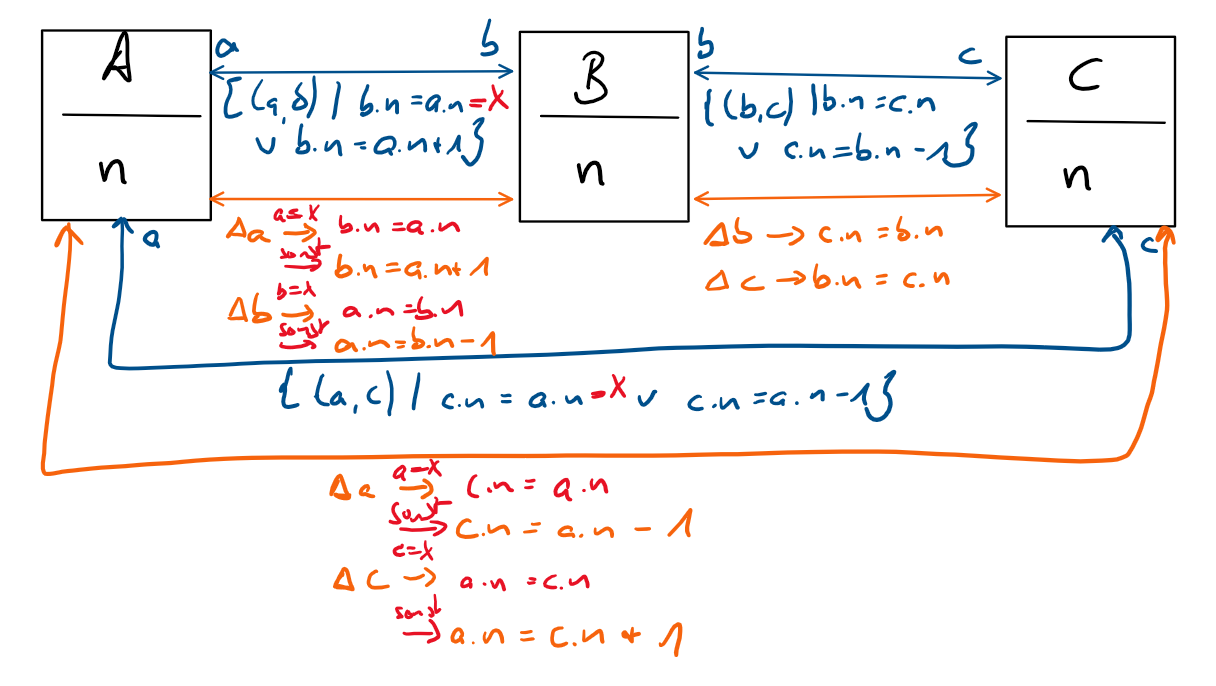
\includegraphics[width=\textwidth]{figures/correctness/orchestration/no_upper_bound_example.png}
    \caption[Example for arbitrary bounds of transformation execution]{Example for an arbitrary bound of necessary transformation execution.}
    \label{fig:orchestration:no_upper_bound}
\end{figure}

\mnote{Generalization to a theoretical incrementation example}
We can generalize the previous example to the one given in \autoref{fig:orchestration:no_upper_bound}.
It is an extension of the example given in \autoref{fig:synchronization:multiple_unidirectional_execution} for the necessity to execute the consistency preservation rules of a bidirectional transformation multiple times.
This also applies to the case in which multiple bidirectional transformations are combined.
The depicted relations and the informally defined consistency preservations rules require that elements \modelelement{A}, \modelelement{B} and \modelelement{C} with the same value of $n$ exist, and that for each \modelelement{A} with value $n$ a \modelelement{B} and \modelelement{C} with $n$ incremented by $1$ exist, except for the case that $n = x-1$.
In consequence, for an \modelelement{A} with $n = i$, all \modelelement{A}, \modelelement{B} and \modelelement{C} with $i \leq n < x$ need to exist.
This, obviously, requires the transformations to be executed $x-1-i$ times.

\mnote{Precise definition of transformation network}
We prove the informally given statement with the following precise definition of the transformations for a variable value of $x$.
Let $\class{A}{}, \class{B}{}, \class{C}{}$ be the classes depicted in \autoref{fig:orchestration:necessity_multiple_executions}.
\begin{align*}
    & 
    \metamodelinstanceset{M}{1} = \mathcal{P}(\metamodelinstances{\class{A}{}}), %\\
    %& 
    \metamodelinstanceset{M}{2} = \mathcal{P}(\metamodelinstances{\class{B}{}}), %\\
    %& 
    \metamodelinstanceset{M}{3} = \mathcal{P}(\metamodelinstances{\class{C}{}}) \\[1em]
    &
    \consistencyrelation{CR}{12} = \setted{\tupled{a,b} \in \metamodelinstances{\class{A}{}} \times \metamodelinstances{\class{B}{}} \mid b.n = a.n + 1 \neq x}, \consistencyrelationset{CR}_{12} = \setted{\consistencyrelation{CR}{12}, \consistencyrelation{CR}{12}^T} \\
    &
    \consistencypreservationrule{\consistencyrelationset{CR}_{12}}^{\rightarrow}(\model{m}{1}, \model{m}{2}, \change{\metamodel{M}{1}}) = \change{\metamodel{M}{2}} \\
    & \formulaskip
    \mathtext{with} \change{\metamodel{M}{2}}(\model{m}{2}) = \setted{b \in \metamodelinstances{\class{B}{}} \mid \exists a \in \change{\metamodel{M}{1}}(\model{m}{1}) : b.n = a.n + 1 \neq x} \\
    & 
    \consistencypreservationrule{\consistencyrelationset{CR}_{12}}^{\leftarrow}(\model{m}{2}, \model{m}{1}, \change{\metamodel{M}{2}}) = \change{\metamodel{M}{1}} \\
    & \formulaskip
    \mathtext{with} \change{\metamodel{M}{1}}(\model{m}{1}) = \setted{a \in \metamodelinstances{\class{A}{}} \mid \exists b \in \change{\metamodel{M}{2}}(\model{m}{2}) : b.n = a.n + 1 \neq x \land a \geq 0} \\
    &
    \transformation{T}_{12} = \tupled{\consistencyrelationset{CR}_{12}, \consistencypreservationrule{\consistencyrelationset{CR}_{12}}^{\rightarrow}, \consistencypreservationrule{\consistencyrelationset{CR}_{12}}^{\leftarrow}} \\[1em]
    & 
    \consistencyrelation{CR}{13} = \setted{\tupled{a,c} \in \metamodelinstances{\class{A}{}} \times \metamodelinstances{\class{C}{}} \mid c.n = a.n}, \consistencyrelationset{CR}_{13} = \setted{\consistencyrelation{CR}{13}, \consistencyrelation{CR}{13}^T} \\
    & 
    \consistencypreservationrule{\consistencyrelationset{CR}_{13}}^{\rightarrow}(\model{m}{1}, \model{m}{3}, \change{\metamodel{M}{1}}) = \change{\metamodel{M}{3}} \\
    & \formulaskip
    \mathtext{with} \change{\metamodel{M}{3}}(\model{m}{3}) = \setted{c \in \metamodelinstances{\class{C}{}} \mid \exists a \in \change{\metamodel{M}{1}}(\model{m}{1}) : c.n = a.n} \\
    & 
    \consistencypreservationrule{\consistencyrelationset{CR}_{13}}^{\leftarrow}(\model{m}{3}, \model{m}{1}, \change{\metamodel{M}{3}}) = \change{\metamodel{M}{1}} \\
    & \formulaskip
    \mathtext{with} \change{\metamodel{M}{1}}(\model{m}{1}) = \setted{a \in \metamodelinstances{\class{A}{}} \mid \exists c \in \change{\metamodel{M}{3}}(\model{m}{3}) : c.n = a.n} \\
    & 
    \transformation{T}_{13} = \tupled{\consistencyrelationset{CR}_{13}, \consistencypreservationrule{\consistencyrelationset{CR}_{13}}^{\rightarrow}, \consistencypreservationrule{\consistencyrelationset{CR}_{13}}^{\leftarrow}} \\[1em]
    &
    \consistencyrelation{CR}{23} = \setted{\tupled{b,c} \in \metamodelinstances{\class{B}{}} \times \metamodelinstances{\class{C}{}} \mid c.n = b.n}, \consistencyrelationset{CR}_{23} = \setted{\consistencyrelation{CR}{23}, \consistencyrelation{CR}{23}^T} \\
    & 
    \consistencypreservationrule{\consistencyrelationset{CR}_{23}}^{\rightarrow}, \consistencypreservationrule{\consistencyrelationset{CR}_{23}}^{\leftarrow} \mathtext{and} \transformation{T}_{23} \mathtext{accordingly} \\[1em]
    &
    \consistencyrelationset{CR} = \consistencyrelationset{CR}_{12} \cup \consistencyrelationset{CR}_{13} \cup \consistencyrelationset{CR}_{23} \\
    &
    \transformationset{T}_{inc} = \setted{\transformation{T}_{12}, \transformation{T}_{13}, \transformation{T}_{23}}
\end{align*}

\mnote{Proof that single execution of each transformation is not sufficient in scenario}
For these transformations, we are able to show that the transformation $\transformation{T}_{12}$ needs to be executed a minimal number of depending on $x$ for a specific input.
Thus, it is not sufficient to execute each transformation only once in this network.

\begin{lemma}[Minimal Number of Transformation Executions]
    \label{lemma:minimal_executions}
    Let $\transformationset{T}_{inc}$ be the previously defined set of transformations and let $\model{m}{1} = \model{m}{2} = \model{m}{3} = \emptyset$ be empty models and $\change{\metamodel{M}{1}} \in \changeuniverse{\metamodel{M}{1}}$ a change with $\change{\metamodel{M}{1}}(\model{m}{1}) = \setted{a \in \metamodelinstances{\class{A}{}} \mid a.n = 0}$.
    Then the result of every orchestration function $\orcfunction{\transformationset{T}_{inc}}$ with $\appfunction{\orcfunction{\transformationset{T}_{inc}}}(\tupled{\model{m}{1},\model{m}{2},\model{m}{3}},\tupled{\change{\metamodel{M}{1}},\identitychange,\identitychange}) \consistenttomath \consistencyrelationset{CR}$ contains $\transformation{T}_{12}$ at least $x-1$ times.
\end{lemma}
\begin{proof}
    $\appfunction{\orcfunction{\transformationset{T}_{inc}}}$ can only return consistent models when it applies the transformations in the order delivered by $\orcfunction{\transformationset{T}_{inc}}$ by definition in \autoref{def:applicationfunction}.
    We thus consider any order of transformations, as delivered by any orchestration function, to show that it contains $\transformation{T}_{12}$ at least $x-1$ times to deliver consistent models.
    
    Let $max_n(\model{m}{1},\model{m}{2},\model{m}{3}) = max\setted{e.n \mid e \in \model{m}{1} \cup \model{m}{2} \cup \model{m}{3}}$ be the maximal value of $n$ in any instance of \modelelement{A}, \modelelement{B} and \modelelement{C} in any given models $\model{m}{1}$, $\model{m}{2}$ and $\model{m}{3}$. In the following, we shortly note $max_n$ if the concrete models are currently not relevant.

    \begin{properdescription}
        \item[Executing $\transformation{T}_{13}$ and $\transformation{T}_{23}$ an arbitrary number of times does not increase $max_n$:]
        The transformations do only ensure that for any given models the returned models contain all elements with the same values of $n$ and do not introduce new elements with values of $n$ larger than the existing ones.
        \item[A single execution of $\transformation{T}_{12}$ increases $max_n$ by at most one:]
        There is no \modelelement{A} or \modelelement{B} with $n > max_n$.
        For every \modelelement{A} with $n < max_n$, $\transformation{T}_{12}$ creates, if necessary, a \modelelement{B} with value $n + 1 \leq max_n$, thus not increasing $max_n$.
        For every \modelelement{B} with $n \leq max_n$, it creates, if necessary, an \modelelement{A} with value $n-1 < max_n$.
        For every \modelelement{A} with $n = max_n$, a \modelelement{B} with value $n+1 = max_n + 1$ is creates, as long as $n \neq x-1$.
        For the newly created \modelelement{B}, no further elements needs to be created to fulfill the consistency relations.
        Thus, $max_n$ is, at most, increased by $1$.
        \item[ When $max_n(\model{m}{1},\model{m}{2},\model{m}{3}) < x-1$, then $\model{m}{1},\model{m}{2},\model{m}{3}$ are not consistent to $\consistencyrelationset{CR}$:]
        There is at least one element within the models with $n = max_n$.
        If the element with $n = max_n$ is an \modelelement{A}, then there must be a \modelelement{B} with value $n+1$, because of $\consistencyrelationset{CR}_{12}$ and because $n < x-1$.
        But since $n = max_n$, such a \modelelement{B} cannot exist, because otherwise $max_n = n+1$, so this is a contradiction.    
        If the element with $n = max_n$ is a \modelelement{C}, then $\consistencyrelationset{CR}_{13}$ requires an \modelelement{A} with the same value of $n$ to exist and the same argument as before leads to a contradiction.
        Finally, if the element with $n = max_n$ is a \modelelement{B}, then because of $\consistencyrelationset{CR}_{23}$ a \modelelement{C} with the same value must exist and then the same argument as before leads to a contradiction.
    \end{properdescription}

    In summary, we have shown that models $\model{m}{1},\model{m}{2},\model{m}{3}$ are only consistent to $\consistencyrelationset{CR}$ when $max_n(\model{m}{1},\model{m}{2},\model{m}{3}) \geq x-1$.
    Additionally, only $\transformation{T}_{12}$ increases $max_n$ and with each execution it only increases it by at most $1$.
    In consequence, starting with $max_n = 0$, we need at least $x-1$ executions of $\transformation{T}_{12}$ in an arbitrary sequence of the transformations in $\transformationset{T}_{inc}$ to achieve consistent models.
\end{proof}

\mnote{Example transformations can force network to perform an arbitrary number of executions}
We have proven that arbitrary transformation networks can require an arbitrary high number of executions of each transformations.
By selecting an appropriate $x$ in the used example network, we can force the network to perform at least $x$ executions of one transformation to yield a consistent tuple of models.
With this insight, it directly follows that we cannot find an approach to define orchestration functions that delivers sequences containing each transformation only once if we want to ensure that if a consistent orchestration of transformations exists, the approach is supposed to deliver it.

\begin{theorem}[Orchestration with Single Execution]
    \label{theorem:orchestration_single}
    For any set of transformations $\transformationset{T}$, there can be models $\modeltuple{m}$ and changes $\changetuple{}$ to them for which each possible orchestration function $\orcfunction{\transformationset{T}}$ with whom $\appfunction{\orcfunction{\transformationset{T}}}(\modeltuple{m}, \changetuple{})$ is consistent, delivers a sequence as $\orcfunction{\transformationset{T}}(\modeltuple{m}, \changetuple{})$ that contains at least one transformation twice.
\end{theorem}
\begin{proof}
    We know from \autoref{lemma:minimal_executions} that $\transformationset{T}_{inc}$ requires at least $2$ executions of $\transformation{T}_{12}$ for the inputs defined in \autoref{lemma:minimal_executions} when selecting $x \geq 3$.
    This proves the theorem by example.
\end{proof}

\mnote{Example generalizes practical scenario, thus single execution not supposed to be sufficient}
We know from \autoref{theorem:orchestration_single} that if we execute each transformation only once, we may exclude cases for which multiple executions of transformations would have led to a consistent tuple of models.
The example we have given in \autoref{fig:orchestration:necessity_multiple_executions} is a simplification of a realistic transformation scenario, which we generalized to the previous network with transformations $\transformationset{T}_{inc}$.
Thus, we can conclude that the insight is potentially relevant for realistic scenarios.
We should not restrict orchestration to execute each transformation only once, as there can be realistic scenarios in which multiple executions are necessary to find consistent models.
In the following, we thus, for first, allow an arbitrary number of executions of each transformation.

% Essential problem: One transformation may restore consistency between A and B and another between A and C. If then a transformation restores consistency between B and C, the resulting B' and C' may not be consistent A anymore.

% \todo{Beispiel warum mehrfache Ausführung nötig, warum also manche Infos erst durch andere bx reinkommen, die bei einer bx isoliert nicht relevant sind.}

% Bestehende Arbeiten (\cite{stevens2020BidirectionalTransformationLarge-SoSym}) schlagen auch vor eine Baumstruktur zu berechnen (Spannbaum), in dem nur entlang der Baumkanten die Transformationen ausgeführt werden. Dies ist jedoch eine starke Einschränkung daran, was die Transformationen ausdrücken können. Betrachtet man beispielsweise PCM, UML und Java, und hat eine Änderung in PCM. Dann könnte der Spannbaum entweder PCM -> UML -> Java sein, oder PCM -> UML + PCM -> Java. In ersterem Fall würde Verhaltensbeschreibung, die von PCM nach Java übertragen, aber in UML nicht dargestellt wird, nicht übertragen. Im zweiten Fall würde zusätzliche Information zwischen UML und Java nicht propagiert (Beispiel?) --> Hier sollte auf das Properties-Kapitel verwiesen werden, wo diese "Bottlenecks" erklärt sein sollten, inklusive einem Beispiel, die allgemein Baumstrukturen für Transformationsnetwerke ausschließen.

% Consequence: We cannot easily restrict the number of allowed executions. We can define networks that require an arbitrary number of executions.
% Also refer to the synchronization example, where we discussed that.
% Let us, for first, assume that transformations need an arbitrary number of executions.


\subsection{Expected Behavior} % Failure Cases} %When to Return $\bot$?}

\mnote{Necessity to define when application function returns $\bot$}
The application function is defined to return models only when they can be derived by applying transformations in an order delivered by the orchestration function and otherwise to return $\bot$.
In addition, we expect a \emph{correct} application function only to deliver models that are consistent.
We did, however, not yet define under which conditions we expect the function not to return $\bot$, because there are different reasons why the function may not be able to deliver consistent models although we could expect it to do so.
In fact, with the current definition, the function is even considered correct if it always returns $\bot$, which is not practical.
Thus, we need to define when exactly we expect the function to return $\bot$.

\mnote{Reasons for not finding an orchestration that yields consistent models}
It might be intuitive to expect an application function to always return consistent models when the input models are consistent and when there is an execution order of the transformations, i.e., an orchestration, that delivers consistent models.
This, in consequence, would lead to the requirement that the orchestration function delivers a sequence of transformations whose application delivers consistent models whenever such a sequence exists for the given models and changes to them.
There can be different reasons why the orchestration function may not deliver such a sequence:
%When is it allowed or needed to return $\bot$?
%It may always return $\bot$ to be correct, this is however not what we want.
%We can distinguish three levels of reasons why the function may not be able to find consistent models:
\begin{properdescription}
    \item[Relations are incompatible:] If the consistency relations are incompatible, a user change may introduce an element for which no consistent models exist. In consequence, the transformation cannot be executed in an order such that the resulting models are consistent and still reflect the given user change.
    %(example with employee for which no consistent other models can be found)
    \item[No orchestration exists:] Even if the relations are compatible, transformations may be defined in a way that they make contradictory decisions for locally consistent solutions. Thus, for a given a change the consistency relations allow different ways to store consistency, of which the transformations always select a way that is not consistent to one of the other relations.
    Then no order of the transformations can restore consistency, although models exist that fulfill consistency for the given change.
    % (example with three options for name mapping with one overlapping, where each transformation always selects the one that is not appropriate for the other). We can further distinguish here whether there is always a change that cannot be processed by a CPR (then the change conflicts with the consistency relations and thus has to be rejected like any change may need to be rejected), or whether an arbitrary long sequence of transformations exists that can be applied but does never yield a consistent set of models.
    \item[No orchestration found:] Finally, although an order of transformations for given changes exists that delivers consistent models, the orchestration function may not deliver it. 
    %finally, the application/orchestration may not be able to find an order of transformations that leads to a consistent state although it exists.
\end{properdescription}

\mnote{Reasons induce each other}
These reasons can be considered at different levels, because each of them induces the next, i.e., if there is no orchestration, it cannot be found, and having contradictory relations, there exists no orchestration for some of the changes.
In the end, all of them lead to the situation that no orchestration can be found and, thus, the orchestration function is not able to deliver it.

\mnote{Compatibility can be assumed, existence of an orchestration cannot}
The initially given intuitive requirement that the orchestration function delivers a consistent orchestration whenever it exists would thus assume that the first two levels do not occur and then require the orchestration function to ensure the third.
While we can assume compatibility of the relations, as we discussed how to analyze it in \autoref{chap:compatibility}, we cannot assume that an orchestration does always exists, as we will see in the following.

\mnote{Compatibility does not ensure existence of orchestration}
Although compatibility reduces the chance that an orchestration function does not deliver a consistent orchestration, as we have motivated with the scenario depicted in \autoref{fig:compatibility:unwanted_behavior}, it does not ensure that there is always such a sequence of transformations that the orchestration function can find.
In general, this is always the case when consistency relations define different options for consistency, i.e., they allow the existence of different corresponding elements to consider the models consistent.
Compatibility ensures that there is an overlap of these corresponding elements, such that for every element, for which consistency is restricted, consistent models can be found.
If, however, the consistency preservation rules of the transformations always restore consistency by introducing corresponding elements that are not in this overlap, each transformation will restore consistency locally to its consistency relation, but they can, together, never restore consistency to all consistency relations.

\mnote{Consistency preservation rules need to select overlapping options in consistency relations}
Consider the situation that we have three metamodels $\metamodel{A}{}$, $\metamodel{B}{}$ and $\metamodel{C}{}$ with instances $\model{a}{i}$, $\model{b}{i}$ and $\model{c}{i}$.
Let us assume that those models are uniquely indexed by $i$ and we defined the following consistency relations:
\begin{align*}
    &
    \consistencyrelation{CR}{AB} = \setted{\tupled{\model{a}{i}, \model{b}{k}} \mid k = i} \\
    &
    \consistencyrelation{CR}{AC} = \setted{\tupled{\model{a}{i}, \model{c}{l}} \mid l = i \lor l = i+1} \\
    &
    \consistencyrelation{CR}{BC} = \setted{\tupled{\model{b}{k}, \model{c}{l}} \mid l = k+1 \lor l = k+2}
\end{align*}
This induces the set of consistent models $\setted{\tupled{\model{a}{i}, \model{b}{k}, \model{c}{l}} \mid  i = k = l-1}$, which is given to all three consistency relations.
Thus for any given model we are able to find instances of the other metamodels that are consistent to all consistency relations.
If we define consistency preservation rules for these consistency relations, the ones for $\consistencyrelation{CR}{AC}$ and $\consistencyrelation{CR}{BC}$ may decide between two models to restore consistency.
If $\consistencyrelation{CR}{AC}$ does always select $\model{c}{i}$ for $\model{a}{i}$ and vice versa, and if $\consistencyrelation{CR}{BC}$ does always select $\model{c}{i+2}$ for $\model{a}{i}$ and vice versa, no orchestration of the transformations will yield consistent models, because they never select those models that are in the overlap of the consistency relations.

\begin{figure}
    \centering
    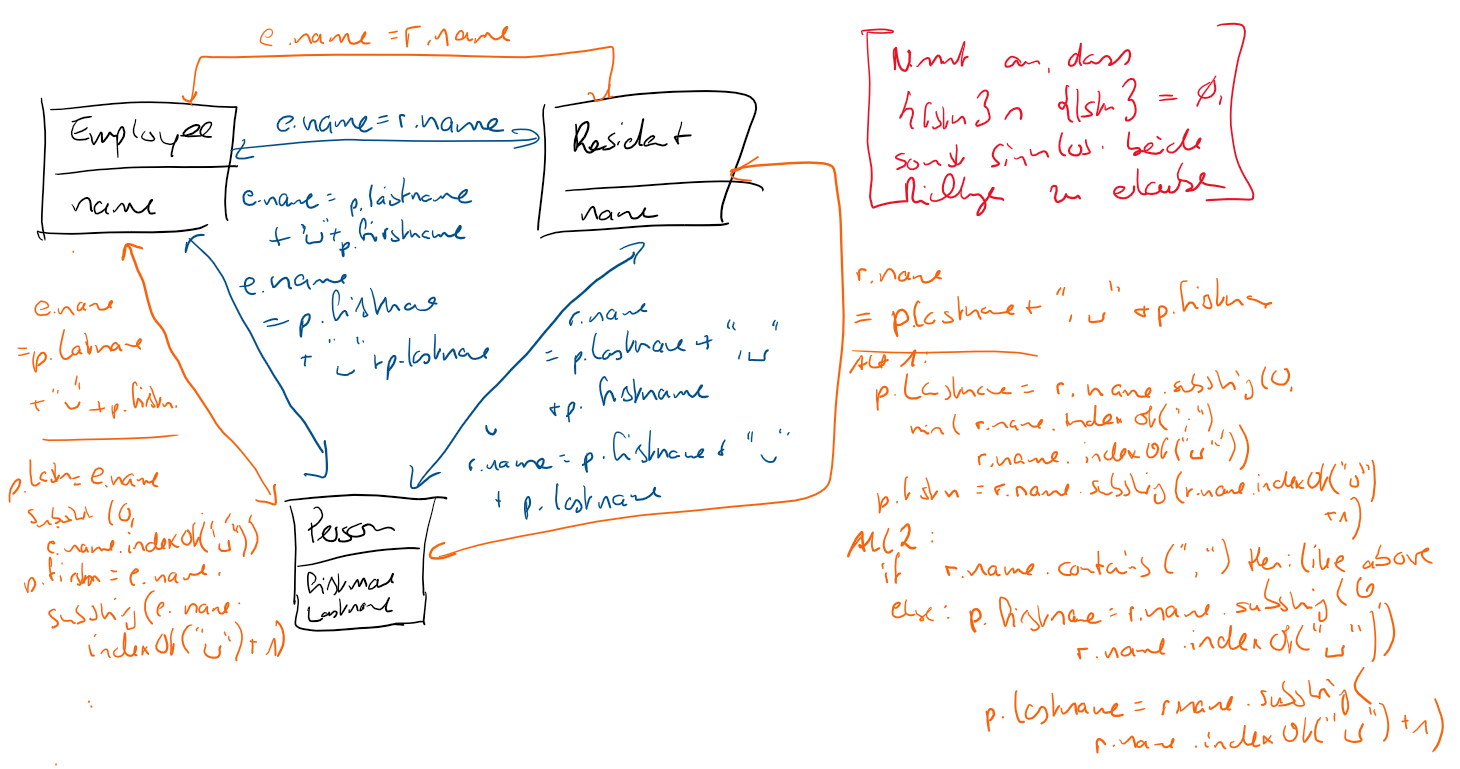
\includegraphics[width=\textwidth]{figures/correctness/orchestration/no_orchestration.png}
    \caption[Consistency preservation rules without orchestration]{Consistency relations with options for corresponding elements leading to consistency preservation rules for which no consistent orchestration exists.}
    \label{fig:orchestration:no_orchestration}
\end{figure}

\mnote{Running example with consistency relations for name composition}
We have already given an abstract example for that problem in \autoref{fig:correctness:no_execution_order}. \autoref{fig:orchestration:no_orchestration}, in addition, demonstrates this situation at a derivation of the running example.
The consistency relation between employees and residents ensures that for each resident and employee there is corresponding other element with the same name.
The consistency relations between employees and persons and between residents and persons ensure that for each person there is a corresponding employee and resident, respectively, but they allow different relations of their names.
While both consider elements corresponding if the name of an employee and resident, respectively, are the concatenation of the first and last name of a person, an employee is also allowed to have the inverse concatenation of last and first name, whereas a resident is also allowed to have this inverse concatenation, but with an additional separation of the last and first name with a comma.
These options for the consistency relations provide further degrees of freedom for each transformation on its own, as they allow, for example, employee names to be encoded differently.
This can, for example, be reasonable if the order of first and last name is not relevant in a model managing employees.
In combination with the other consistency relations, however, the only employees, residents and persons that are considered consistent to all of the consistency relations are those having the same names with the concatenation of first and last name.
Nevertheless, these consistency relations are compatible, because for each possible condition element, i.e., for every possible employee, person and resident, there are consistent models that contain them.

\mnote{Relations in the running example without consistent orchestration}
Consistency relations that preserve these consistency relations need to to choose one of the given options for the names of corresponding employees, residents and persons.
\autoref{fig:orchestration:no_orchestration} sketches consistency preservation rules that make such a selection.
The rules with alternative 1 ensure that for each employee, resident and persons corresponding elements exist, which fulfill those relations of the names that are conflicting.
This means, the employee name is the concatenation of the last and first name of a person, whereas the resident name contains an additional comma in that concatenation.
In the other direction, the names of employees and residents are split at the appropriate indices, given by the whitespace and comma, respectively, to calculate the required first and last name of a person.
In consequence, there is no execution sequence of the transformations that results in consistent models, because the execution of the transformation between employees and persons always leads to a violation of the consistency relation between residents and persons and vice versa.
This is because the transformation between person and resident always introduces a comma in the resident name, which is then appended to the last name by the transformation between employee and persons.
A repeated execution of the transformation repeatedly appends that comma.
On the other hand, the execution of any of the transformation does never lead to the introduction of a person that fulfills the non-conflicting conditions of both consistency relations by simply containing a first and last name, which is represented as concatenation of first and last name in both an employee and resident.
This is concrete example for the previously discussed abstract situation that of different options in consistency relations always the non-overlapping ones are chosen by the consistency preservation rules.

\mnote{Alternative relations in the running example}
If we consider the alternative 2 for the consistency preservation rule between persons and residents, we can always find a consistent orchestration.
The alternative rule decides how consistency is ensured based on the existence of a comma within the resident name.
If a comma is present, the name relation containing a comma is used, and otherwise the simple concatenation of first and last name is assumed.
For an employee, first execution the transformation from employees to residents and afterwards the one from residents to persons ensures that all consistency relations are fulfilled, because the one between residents and persons sets first and last name of a person according to the relations that is also fulfilled between person and employee, because the name does not contain a comma.
For a person, first executing the transformation from persons to employees and then following the process above also ensures consistency.
Finally, for a resident, we can, for example, first apply the transformation between residents and employees and then the one between residents and persons, resulting in consistent models due to the same reasons as above.

\mnote{Only specific orchestrations yield consistent models}
Although there are consistent orchestration of the transformations with the consistency preservation rule defined as alternative 2, not every execution order leads to consistent models.
In the scenarios discussed above, we have ensured that the transformation between residents and persons is executed for a resident first.
If that transformation is first executed for a person, then a comma is added, which leads to the subsequent application of the same consistency preservation rules as with alternative 1, meaning that no further orchestration yields consistent models.

\mnote{Necessity to find consistent orchestrations}
No matter whether exactly those consistency relations and preservation rules for them may occur in an actual transformation network, they exemplify the general situation of having consistency preservation rules that select one of different options provided by the consistency relation to introduced corresponding elements to restore consistency.
The example shows that whether or not a consistent orchestration of transformations exists in such a situation depends on whether at least one transformation selects an option that is consistent to other consistency relations as well.
It also shows that even if a consistent orchestration exists, not all orchestrations yield consistent models, thus we need to be able to find one that does.

\mnote{Resolvability as the existence of an orchestration}
In accordance with existing work \cite{stevens2020BidirectionalTransformationLarge-SoSym}, we call a given set of models and changes \emph{resolvable} by a transformation network, if an orchestration exists.
In contrast to existing work, we do, however, not restrict ourselves to a single execution of each transformation, as we have motivated before.

\mnote{Necessity to deal with unresolvability}
We have to accept that transformation networks may be unresolvable, i.e., that there is no consistent orchestration of the transformations.
Ensuring that a network is resolvable for any changes would lead to restrictions for the individual transformations, which would especially require different transformations to be aligned with each other.
Since that conflicts our assumption of independent development and modular reuse, we do not focus on that problem, but accept that it can occur and instead focus on how we can find an orchestration if it exists. 

\mnote{Optimality property of orchestration function}
In conclusion, we expect the application function to deliver consistent models whenever a consistent orchestration, i.e., an execution order that yields consistent models, exists.
Thus, we want to ensure that the orchestration function is able to always find such an orchestration, if it exists.
We define this as an \emph{optimality} property in the following.

% "has a resolution" bei Stevens entspricht im Prinzip Kompatibilität
% "is resolvable" bei Stevens entspricht im Prinzip "orchestration exists"

% In accordance to existing work, such as \cite{stevens2020BidirectionalTransformationLarge-SoSym}, we call a given set of models and changes \emph{resolvable} by the transformation network, if there exists a sequence of the transformations such that the resulting models are consistent.
% We do, however, not restrict ourselves to a single execution of each transformation but allow them to be executed multiple times (as motivated before).
% Orchestration ermittelt eine "Resolution" (siehe bestehende Arbeiten~\cite{stevens2020BidirectionalTransformationLarge-SoSym}), also eine Ausführungsreihenfolge, zumindest wenn man sie als "korrekt" bezeichnet.

% Argumentation:
% Compatibility können wir fordern, dass eine Orchestrierungsstrategie existiert aber nicht. 

% We can avoid the first by requiring compatibility.
% We need to make restrictions to the transformation to resolve the second. We do, however, probably need to require them to know about the other transformations to avoid that. Finally, we will have to deal with that situation and then inform the user about the problem.
% We investigate whether we can always guarantee to find an orchestration if it exists.
% For now, we focus on the last problem, since that is a problem of the application and orchestration function, rather than the problem that no orchestration may exist at all.

% DECIDED THAT THE FOLLOWING IS NOT AN OPTINO BUT THE SECOND IS DEFINITE.
% Now we have these options:
% \begin{itemize}
%     \item We accept that there is no orchestration or that the strategy does not find it in specific situations, than we only need to consider that the strategy must always terminate.
%     We could, for example, change the algorithm such that it always returns $\bot$, which is correct, or terminates after executing each transformation once.
%     \item We define a precise criterion when the strategy is allowed to return $\bot$. Most intuitively, one might say that it should only return $\bot$ whenever no orchestration exists.
% \end{itemize}



\subsection{Optimal Orchestration}

% An application function that delivers consistent models whenever an orchestration exists that yields them is what we would assume \emph{optimal}.
% Recall that $\generalizationfunction{\metamodeltuple{M},\transformation{t}}$ is the generalization function that applies a transformation, which is only defined for two models, to a model tuple that instantiate all metamodels in $\metamodeltuple{M}$.

% \begin{definition}[Optimal Transformation Application Function]
%     Let $\transformationset{T}$ be a set of transformations for a set of metamodels $\metamodeltuple{M} = \tupled{\metamodelsequence{M}{n}}$.
%     We say that an application function $\appfunction{\orcfunction{\transformationset{T}}}$ for these transformations is \emph{optimal} if it returns models that are consistent whenever there is an orchestration of the transformation that yields a consistent set of models whenever it exists, i.e.,
%     \begin{align*}
%         &
%         \forall \modeltuple{m} \in \metamodeltupleinstanceset{M} : \forall \changetuple{\metamodeltuple{M}} = \tupled{\change{\metamodel{M}{1}}, \dots, \change{\metamodel{M}{n}}} \in \changeuniverse{\metamodeltuple{M}} :
%         \modeltuple{m} \consistenttomath \consistencyrelationset{CR} \Rightarrow \\
%         & \formulaskip
%         \bigl(
%             \exists \transformation{t}_{1}, \dots, \transformation{t}_{m} \in \transformationset{} : 
%             \exists \changetuple{\metamodeltuple{M}}' = \tupled{\change{\metamodel{M}{1}}', \dots, \change{\metamodel{M}{n}}'} \in \changeuniverse{\metamodeltuple{M}} :\\
%             & \formulaskip \formulaskip
%             \generalizationfunction{\metamodeltuple{M}, \transformation{t}_{1}} \concatfunction \dots \concatfunction \generalizationfunction{\metamodeltuple{M}, \transformation{t}_{m}}(\modeltuple{m}, \changetuple{\metamodeltuple{M}}) = (\modeltuple{m}, \changetuple{\metamodeltuple{M}}')\\
%             & \formulaskip \formulaskip
%             \land \tupled{\change{\metamodel{M}{1}}'(\model{m}{1}), \dots, \change{\metamodel{M}{n}}'(\model{m}{n})} \consistenttomath \consistencyrelationset{CR} \bigr) \\
%             & \formulaskip
%             \Rightarrow \appfunction{\orcfunction{\transformationset{T}}}(\modeltuple{m},\changetuple{\metamodeltuple{M}}) \consistenttomath \consistencyrelationset{CR}
%         \bigr)
%     \end{align*}
% \end{definition}

\mnote{Definition of optimal orchestration function}
To ensure that an application function delivers consistent models whenever a consistent orchestration exists, we need to find an orchestration function that fulfills this property.
We denote this as an \emph{optimal} orchestration function.
Recall that $\generalizationfunction{\metamodeltuple{M},\transformation{t}}$ is the generalization function that applies a transformation, which is only defined for two models, to a model tuple that instantiate all metamodels in $\metamodeltuple{M}$.
% It is obvious that we can define consistency preservation rules for which the orchestration function cannot find an execution order that returns a consistent tuple of models after certain changes. We already gave an example in \autoref{fig:correctness:no_execution_order}. There exists no execution order for any input value that terminates. The transformations will always increase the value, although the defined relations could be fulfilled for the input value, but the transformations never find that solution.

% Although we will discuss restrictions to relations and transformations that reduce the chance that no solution can be found, it will not be possible to ensure that such a solution can always be found. This is due to the reason that transformations can perform arbitrary changes given that transformations are Turing complete, which should not be restricted, because it is unclear which restrictions could be made without forbidding scenarios that should actually we supported. Thus, we assume that transformations are Turing complete.

% We explicitly allow the orchestration function to return a sequence that will, if applied to models and changes to them, not deliver a consistent tuple of models. As discusses, this is supposed to reflect cases in which no such sequence can be calculated.
% However, it may be useful to have some notion of \emph{optimality} that ensures that if a sequence that delivers a consistent result exists, the orchestration function is supposed to find it.
% Formally, this notion looks as follows.

\begin{definition}[Optimal Transformation Orchestration Function]
    Let $\transformationset{T}$ be a set of transformations for a set of metamodels $\metamodeltuple{M} = \tupled{\metamodelsequence{M}{n}}$.
    We say that an orchestration function $\orcfunction{\transformationset{T}}$ for these transformations is \emph{optimal} if it returns a consistent orchestration whenever it exists, i.e.,
    \begin{align*}
        &
        \forall \modeltuple{m} \in \metamodeltupleinstanceset{M} : \forall \changetuple{\metamodeltuple{M}} = \tupled{\change{\metamodel{M}{1}}, \dots, \change{\metamodel{M}{n}}} \in \changeuniverse{\metamodeltuple{M}} :
        \modeltuple{m} \consistenttomath \consistencyrelationset{CR} \Rightarrow \\
        & \formulaskip
        \bigl[ \bigl(
            \exists \transformation{t}_{1}, \dots, \transformation{t}_{m} \in \transformationset{} : 
            \exists \changetuple{\metamodeltuple{M}}' = \tupled{\change{\metamodel{M}{1}}', \dots, \change{\metamodel{M}{n}}'} \in \changeuniverse{\metamodeltuple{M}} :\\
            & \formulaskip \formulaskip
            \generalizationfunction{\metamodeltuple{M}, \transformation{t}_{1}} \concatfunction \dots \concatfunction \generalizationfunction{\metamodeltuple{M}, \transformation{t}_{m}}(\modeltuple{m}, \changetuple{\metamodeltuple{M}}) = (\modeltuple{m}, \changetuple{\metamodeltuple{M}}')\\
            & \formulaskip \formulaskip
            \land \tupled{\change{\metamodel{M}{1}}'(\model{m}{1}), \dots, \change{\metamodel{M}{n}}'(\model{m}{n})} \consistenttomath \consistencyrelationset{CR} \bigr) \\
            & \formulaskip
            \Rightarrow \bigl(        
            \exists \transformation{t}_{1}', \dots, \transformation{t}_{m}' \in \transformationset{} : 
            \exists \changetuple{\metamodeltuple{M}}'' = \tupled{\change{\metamodel{M}{1}}'', \dots, \change{\metamodel{M}{n}}''} \in \changeuniverse{\metamodeltuple{M}} :\\
            & \formulaskip \formulaskip
            \orcfunction{\transformationset{T}}(\modeltuple{m}, \changetuple{\metamodeltuple{M}}) = \tupled{\consistencypreservationrule{1}', \dots, \consistencypreservationrule{m}'} \\
            & \formulaskip \formulaskip
            \land \generalizationfunction{\metamodeltuple{M},\transformation{t}_{1}'} \concatfunction \dots \concatfunction \generalizationfunction{\metamodeltuple{M},\transformation{t}_{m}'}(\modeltuple{m}, \changetuple{\metamodeltuple{M}}) = (\modeltuple{m}, \changetuple{\metamodeltuple{M}}'')\\
            & \formulaskip \formulaskip
            \land \tupled{\change{\metamodel{M}{1}}''(\model{m}{1}), \dots, \change{\metamodel{M}{n}}''(\model{m}{n})} \consistenttomath \consistencyrelationset{CR}
        \bigr) \bigr]
    \end{align*}
\end{definition}

\mnote{Optimal orchestration function not restricted to return sequence only when it yields consistent models}
Note that we do not require an optimal orchestration function not to return a sequence when there is no consistent orchestration.
This is reasonable, because an application function may be defined to return consistent models whenever there is a consistent orchestration, but to also support the process of identifying why there is none by delivering a sequence of transformations that leads to a failure.

\mnote{Optimality of the application function}
Finally, the result of the application function is what is relevant in the process of consistency preservation in a transformation network.
Thus, we apply the notion of \emph{optimality} to that function accordingly by requiring it to deliver consistent models whenever a consistent orchestration exists.

\begin{definition}[Optimal Transformation Application Function]
    \label{def:optimalapplicationfunction}
    Let $\transformationset{T}$ be a set of transformations for a set of metamodels $\metamodeltuple{M} = \tupled{\metamodelsequence{M}{n}}$.
    We say that an application function $\appfunction{\orcfunction{\transformationset{T}}}$ for these transformations is \emph{optimal} if it returns models that are consistent whenever there is a consistent orchestration of the transformation, i.e.,
    \begin{align*}
        &
        \forall \modeltuple{m} \in \metamodeltupleinstanceset{M} : \forall \changetuple{\metamodeltuple{M}} = \tupled{\change{\metamodel{M}{1}}, \dots, \change{\metamodel{M}{n}}} \in \changeuniverse{\metamodeltuple{M}} :
        \modeltuple{m} \consistenttomath \consistencyrelationset{CR} \Rightarrow \\
        & \formulaskip
        \bigl(
            \exists \transformation{t}_{1}, \dots, \transformation{t}_{m} \in \transformationset{} : 
            \exists \changetuple{\metamodeltuple{M}}' = \tupled{\change{\metamodel{M}{1}}', \dots, \change{\metamodel{M}{n}}'} \in \changeuniverse{\metamodeltuple{M}} :\\
            & \formulaskip \formulaskip
            \generalizationfunction{\metamodeltuple{M}, \transformation{t}_{1}} \concatfunction \dots \concatfunction \generalizationfunction{\metamodeltuple{M}, \transformation{t}_{m}}(\modeltuple{m}, \changetuple{\metamodeltuple{M}}) = (\modeltuple{m}, \changetuple{\metamodeltuple{M}}')\\
            & \formulaskip \formulaskip
            \land \tupled{\change{\metamodel{M}{1}}'(\model{m}{1}), \dots, \change{\metamodel{M}{n}}'(\model{m}{n})} \consistenttomath \consistencyrelationset{CR} \bigr) \\
            & \formulaskip
            \Rightarrow \appfunction{\orcfunction{\transformationset{T}}}(\modeltuple{m},\changetuple{\metamodeltuple{M}}) \consistenttomath \consistencyrelationset{CR}
        \bigr)
    \end{align*}
\end{definition}

\mnote{Optimal application function requires optimal orchestration function}
According to the defined behavior of an application function, an optimal applicaion function requires an optimal orchestration function.

\begin{lemma}[Optimal Application Function]
    \label{lemma:optimalapplicationfunction}
    An application function $\appfunction{\orcfunction{\transformationset{T}}}$ can only be optimal if $\orcfunction{\transformationset{T}}$ is optimal.
\end{lemma}
\begin{proof}
    Let us assume that the complete condition in \autoref{def:optimalapplicationfunction} is fulfilled, i.e., that the input models are consistent and that there is consistent orchestration of the transformations.
    Then to be optimal, the application function needs to return models that are consistent.
    According to the definition of an application function (see \autoref{def:applicationfunction}), the sequence of transformations delivered by $\orcfunction{\transformationset{T}}$ for that input must yield the same model tuple as $\appfunction{\orcfunction{\transformationset{T}}}$.
    Thus, the orchestration function must deliver a sequence for such inputs that yields consistent models, which is equivalent to $\orcfunction{\transformationset{T}}$ being optimal.
\end{proof}

\mnote{Different approaches to achieve optimality}
We can distinguish two approaches to ensure that the orchestration function is optimal, i.e., that it does always find a consistent orchestration if it exists.
Let $P_{i}$ be the problem space, i.e., all possible transformation execution orders for an input $i$ of models and a change to them and let $S_{i}$ be the solution space with those orders that yield consistent models.
\begin{properdescription}
    \item[Strategy Definition:] Define a strategy that explores the problem space $P_{i}$ to find one of the sequences in the solution space $S_{i}$, if $S_{i} \neq \emptyset$.
    \item[Transformation Restriction:] Define a \emph{well-behavedness} property for the transformations that ensures that executing the transformations in any order often enough, they yield consistent models if $S_{i} \neq \emptyset$, i.e., for any given input $i$ there is an $n \in \mathbb{N}$ such that $\forall s \in P_{i} : \abs{s} > n \Rightarrow s \in S_{i}$.
\end{properdescription}

%Unfortunately, optimality is a property that we cannot request from an orchestration function. Optimality would mean that the orchestration function can decide whether there is sequence of transformations that leads to consistent models and thus terminate.

\mnote{No restrictions to transformations}
In the latter case, the orchestration function may return any order of the transformations, as long as the sequence is long enough to be optimal.
This means, performing an iterative execution of the transformations leads to a consistent result, comparable to a fixed-point iteration.
Since optimality is a property of an orchestration function with respect to a set of transformations, defining a \emph{well-behavedness} property as a restriction for transformations to easy finding an optimal orchestration function will potentially not concern a single transformation but the set of them.
This can easily contradict our assumption of independent development and reuse or lead to restrictions of transformation that are not practical anymore.
Thus, we first follow the former approach and investigate the possibility to find an optimal orchestration function without restricting the transformations.
%Optimality of an orchestration function means that it can decide whether there is a sequence of transformations that leads to consistent models and thus terminates.
In the following, we therefore define a general algorithm that realizes an application function and investigate how we can ensure that its orchestration function is optimal.
